\chapter{Results}\label{ch:results}

\section{modelling}
% hier steeds het discrete model en het HGO model vergelijken! dit is niet overal toepasbaar maar als het toepasbaar is, is dit wel de beste structuur om ook gelijk de verschillen inzichtelijk te maken tussen de twee modellen

\subsection{Influence fiber bonding}\label{sec:results_fiber_bonding}
\subsection{Influence force direction}\label{sec:results_force_direction}
Matching the magnitude of the normal and tangential force components is also described by...
\subsection{Behavioral adaptions}\label{sec:results_behavioral_adaptions}
\subsection{Influence fiber stiffness}\label{sec:results_fiber_stiffness}
\subsection{Influence fiber density}\label{sec:results_fiber_density}
\subsection{}\label{sec:results_}
\subsection{}\label{sec:results_}
\subsection{}\label{sec:results_}









% - De krachten die ook daadwerkelijk op de kikker staan nemen en kijken welke contactkrachten dit oplevert 
% % dit nog doen!
% - vervolgens checken of deze krachten laag genoeg zouden zijn om ahesie te behouden uitgaande van capilaire adhesie met hondert procent contactoppervlak




% The results of the model visible in Figure \ref{fig:coarse_fibers} clearly show that the stress is strongly influenced by the location of the fiber re-enforcement. This is also visible for the results of the model with the small fibers but the variation in stress is much less for this model. The most important observation is that both fibre re-enforced models have a much lower value for the stress at the end of the geometry at $L = 10 \mu m$ on the horizontal axis. This reduction in peak stress increases the adhesive strength of the material. 

% \begin{figure}[h!]
%     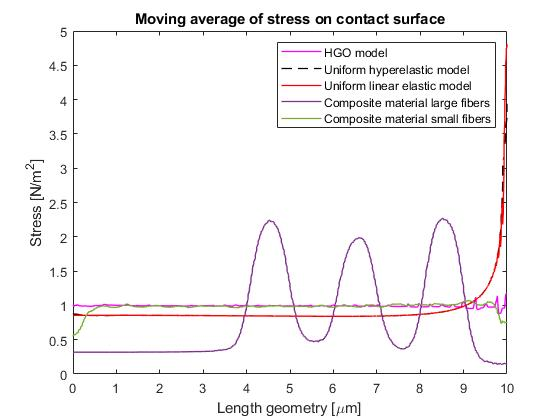
\includegraphics[width=\linewidth, height=6cm, angle=0]{Pictures/validation/validatie_matlab_plot.jpg}
%     \caption{Stress in the different models used for the validation. The average stress is equal for all the models.}
%     \label{fig:matlab_validation_stress}
% \end{figure}


% \section{Experimental testing}

% \begin{figure}[h!]
%     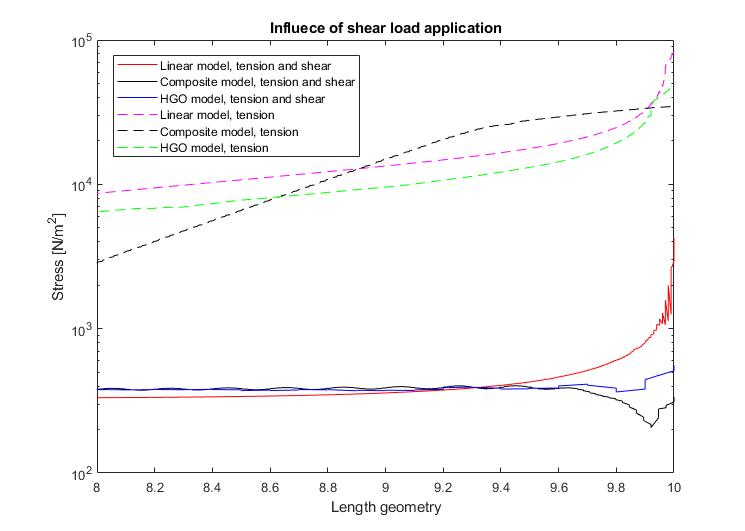
\includegraphics[width=\linewidth, height=6cm, angle=0]{Pictures/validation/comparison_all_data.jpg}
%     \caption{Stress in the contact surface for a geometry loaded with a shear force and a perpendicular force. The x-axis represents the corner of the geometry which is the location of the relevant material behaviour.}
%     \label{fig:validation_shear}
% \end{figure}



% \begin{figure}[h!]
%     \includegraphics[width=\linewidth, height=6cm, angle=0]{Pictures/validation/test_geometry_boundaries.png}
%     \caption{Simple geometry for model testing and validation. The upper red boundary is subjected to the shear  and perpendicular forces which are represented by $F_t$ and $F_n$ respectively. The lower blue boundary is fixed and the green side boundaries are free. Stress measurements are performed on the blue boundary.}
%     \label{fig:test_geometry}
% \end{figure}